\documentclass{article}
\usepackage{iclr2027_conference,times}
\usepackage[T1]{fontenc}
\usepackage[utf8]{inputenc}
\usepackage{amsmath,amssymb,booktabs,graphicx,microtype,url}
\usepackage{pgfplots}
\pgfplotsset{compat=1.18}
\usepackage{hyperref}
\hypersetup{hidelinks,pdftitle={From Detection Scores to Auditable Explanations},pdfauthor={Research revision}}
\title{From Detection Scores to Auditable Explanations:\\A Reproducibility Study of Face Forgery Detectors}
\author{Research revision for author review\\Not submitted; image-level explanation experiments pending}
% The official template's review/acceptance banner must not imply a submission.
\iclrfinalcopy
\makeatletter
\def\iclr@conference{Research revision, 11 September 2026; not submitted}
\makeatother
\newcommand{\AUC}{\operatorname{AUC}}
\newcommand{\BA}{\operatorname{BA}}
\newcommand{\ind}{\mathbb{1}}
\newcommand{\todoexperiment}{\textbf{Not executed on the full image cohort.}}
\begin{document}
\maketitle
\begin{abstract}
Explanations of face forgery detectors are meaningful only when model provenance, sample identity, decision rules, and attribution coordinates are reliable. We audit a released spatial--spectral benchmark and reanalyse 54 prediction exports from six RGB detector families and three random seeds on validation, clean-test, and degraded-test partitions of MFFI. The released fine-tuned checkpoints are not the same experimental regime as the earlier scratch/frozen-backbone manuscript. We additionally identify an identical duplicated observation and a missing image in every RGB validation export, and disclose the derived 147,362-image view used for threshold calibration. On 181,947 test images, DINOv3 has the highest mean clean ROC-AUC within the released RGB roster (0.933), whereas the CLIP-based detector leads under degradation (0.742). With validation-selected decision thresholds, errors shared by all six seed-42 RGB checkpoints increase from 3.09\% on clean images to 11.26\% on degraded images; the corresponding 18-checkpoint intersections are 1.53\% and 5.43\%. We specify reproducible protocols for an identical confusion-stratified 64-image cohort, native-coordinate spatial--frequency comparisons, and complete-roster shared-error analysis. The contribution is an auditable prediction-level reanalysis and an explanation protocol, not a completed visual or causal explanation study: full-cohort heatmaps and image-level reproduction remain pending authenticated source-image access.
\end{abstract}

\section{Introduction}
Face forgery detection is often summarized by a ranking of classifiers. That ranking does not by itself reveal whether models share blind spots, whether spectral representations expose useful manipulation evidence, or whether an attribution map faithfully reflects a decision. A visually plausible heatmap can be insensitive to learned parameters \citep{adebayo2018}; deleting apparently important pixels can introduce a distribution shift that confounds explanation evaluation \citep{hooker2019}. These concerns are especially important when a study combines different input representations, pretraining regimes, architectures, and explanation methods.

The present work revisits the released artifacts accompanying the MFFI benchmark study of \citet{cunha2026}. That earlier manuscript reports predominantly scratch-trained detectors and a frozen DINOv3 backbone. The checkpoint release inspected here is predominantly fine-tuned and includes a ConvNeXt-based DINOv3 model. We therefore do not describe the released weights as a reproduction of the earlier table, compare the two as a controlled pretraining ablation, or reuse its four illustrative attribution examples as new experimental evidence.

Our focus is the chain of evidence linking a checkpoint to a prediction, a prediction to a source image, and an attribution to a fixed mathematical target. This perspective exposes an otherwise easy-to-miss validation-export defect, separates architecture from training-regime claims, and makes shared failures measurable without inventing their causes. It also resolves two ambiguities in common explanation protocols: the same 64 images cannot generally be balanced in every model's confusion matrix, and a location in a Fourier map is not a location on a face.

The contributions are threefold. First, we provide a provenance-aware reanalysis of released RGB predictions with explicit validation curation, frozen thresholds, and seed-level reporting. Second, we quantify complete-roster shared errors and their sensitivity to degradation and roster size. Third, we define executable, evidence-preserving explanation protocols that distinguish completed numerical results from image-dependent experiments that have not yet been run. This is a reproducibility and diagnostic study; it does not introduce a new detector or assert state-of-the-art performance.

\section{Related work and methodological basis}
\paragraph{Frequency evidence is not automatically robust evidence.}
MFFI was introduced to evaluate face forgery detection across diverse sources and degradations \citep{miao2025}. Frequency-based detection is motivated by discrepancies between generated and natural images \citep{frank2020}. More recent work shows that detectors can themselves become biased toward particular frequency bands: FreqDebias combines frequency-diversifying augmentation and consistency regularization to mitigate that dependence \citep{kashiani2025}. Consequently, observing a spectral activation cluster is not sufficient evidence of manipulation localization, generalization, or a causal forensic cue. Our comparisons use matched, separately trained representations and select the architecture pair using validation information rather than the test ranking.

\paragraph{Attribution methods answer different questions.}
Integrated Gradients (IG) attributes a fixed scalar output relative to a baseline along a path \citep{sundararajan2017}; Grad-CAM constructs a gradient-weighted localization map at a specified layer \citep{selvaraju2017}. LIME fits a local surrogate \citep{ribeiro2016}, whereas Kernel SHAP estimates coalition contributions under a Shapley-oriented weighting scheme \citep{lundberg2017}. Attention rollout propagates attention connectivity and is retained here as a class-agnostic diagnostic rather than equated with a class-specific explanation \citep{abnar2020}. Applying all these methods does not produce independent confirmations of a hypothesis because methods share models, inputs, baselines, and sometimes failure modes.

\paragraph{Recent explanation research strengthens the evaluation requirements.}
Quantus emphasizes evaluation across multiple explanation properties \citep{hedstrom2023}. Manifold IG addresses limitations of conventional straight-line attribution paths \citep{zaher2024}; coalition-attribution research shows that partitioning inputs changes the attribution question \citep{zheng2025}. Pixel-level certification requires more than applying a smoothing heuristic \citep{anani2025}. FocusViT further combines class-specific gradient information with validation-based layer aggregation for transformers \citep{ali2026}. These studies inform our controls and limitations. We do not claim to implement manifold IG, certified attribution, or FocusViT, and do not select explanation layers on the 64-image test cohort.

\section{Artifact audit and evaluation protocol}
\subsection{Immutable scope and training provenance}
The source baseline is the repository's \texttt{ICLR} commit beginning \texttt{1643db7a}; the inspected model release is pinned to the full immutable revision listed in Appendix~\ref{app:reproduce}. The primary quantitative roster contains ResNet, Xception, MobileNet, ViT, CLIP, and DINO, each with RGB inputs and seeds 42, 123, and 2024. We inspect validation, clean-test, and degraded-test predictions for all 18 checkpoints, yielding 54 exports. We use the release's family labels without implying that they uniquely identify architecture or training history. In particular, the released DINO model is a fine-tuned ConvNeXt backbone, not the frozen transformer described in the earlier manuscript.

The broader validation-selection screen comprises the six families, seven representations, and these same three seeds. Its 126 configurations supply released aggregate validation AUC values for representation selection; those aggregates must be distinguished from the 54 RGB prediction files independently reanalysed here. Inactive metadata fields are not treated as proof of checkpoint topology. A reproducible loader must reconstruct the architecture from the recorded regime and checkpoint structure, load the complete state strictly, and avoid downloading unrelated initial weights before loading a full checkpoint.

\subsection{Identity integrity and explicit validation curation}
We validate identifiers, label agreement, finite probabilities in $[0,1]$, duplicate records, and complete expected test coverage before computing metrics or intersections. Every RGB validation export contains 147,363 rows but repeats ID 131900 and omits ID 131899. The two repeated rows are identical within each export. The supplied manifest identifies the repeated observation as fake and the missing observation as real. This pattern is consistent with a failed-image substitution mechanism, but the exported records alone do not establish the original cause.

We preserve the raw exports. A separate, explicitly requested derived view removes only identical duplicates, records rather than imputes the missing observation, and requires the same observed ID set across all compared validation files. The resulting validation population has 147,362 images. Non-identical duplicates, label disagreement, or inconsistent missingness cause failure instead of automatic repair. The clean and degraded test exports each contain 181,947 unique observations, with 77,602 real and 104,345 fake labels, matching the supplied test manifest.

The legacy exports identify observations numerically rather than by source-file hashes. Mapping these numbers to filenames therefore depends on the supplied original manifest order. Matching ID sets and labels is necessary but cannot prove byte-level source-image identity. We record the manifest hash and this assumption, and require a future image-level rerun to reproduce probabilities and decisions before accepting attribution outputs as belonging to these predictions. The main numerical results concern exported predictions; they are not represented as independent inference reproduction.

\subsection{Calibration, metrics, and uncertainty}
Let $p_{mi}$ be the exported fake-class probability of model $m$ on observation $i$, with $y_i=1$ indicating fake. For each checkpoint, we choose a threshold using only its derived validation predictions:
\begin{equation}
 t_m=\arg\max_{t\in\mathcal{T}_m}\BA\bigl(y,\ind[p_m\ge t]\bigr),\qquad
 \BA=\tfrac12(\mathrm{TPR}+\mathrm{TNR}),
\end{equation}
where candidate thresholds are observed probabilities together with 0, 0.5, and 1; ties use the smallest threshold. We freeze $t_m$ for clean and degraded test evaluation. This standardized rule differs from heterogeneous threshold policies embedded in some released summaries. It does not affect ROC-AUC, but it does affect confusion strata and shared-error counts.

We report ROC-AUC and balanced accuracy, and retain average precision, class-conditional error rates, F1, MCC, Brier score, and a specified-bin calibration diagnostic in machine-readable outputs. Mean and sample standard deviation across three training seeds describe variation among these runs; three seeds do not characterize all training uncertainty. Any image-resampling confidence interval is conditional on fixed checkpoints and the stated linkage assumption. It must not be confused with seed uncertainty, identity-cluster uncertainty, or evidence of cross-dataset generalization. No formal superiority claim is based solely on a small difference of means.

\subsection{Definition of shared errors}
For a frozen roster $\mathcal{M}$, define
\begin{equation}
 H(\mathcal{M})=\{i:\ \forall m\in\mathcal{M},\ \ind[p_{mi}\ge t_m]\ne y_i\}.
\end{equation}
The primary roster uses the six seed-42 RGB checkpoints. A separate sensitivity analysis uses all 18 RGB checkpoints. Both require complete predictions on exactly the same population. Missing records are neither counted as errors nor silently removed by an inner join. An empty intersection is a legitimate outcome. The term \emph{shared error} refers only to the declared roster; it does not mean an image defeats every possible network, representation, seed, or future detector.

\section{Explanation protocols}
\subsection{Task 1: one reproducible 64-image diagnostic cohort}
The reference checkpoint is ResNet/RGB/fine-tuned/seed 42, fixed before inspecting heatmaps. With global sampling seed 42, we sample without replacement exactly 16 true positives, 16 false negatives, 16 true negatives, and 16 false positives from the clean test predictions of this reference. The 64 IDs and their order are frozen and reused for every evaluated model. Each model retains its own prediction and confusion outcome; only the reference is guaranteed to have the balanced $16\times4$ matrix. Insufficient reference-stratum counts raise an error rather than changing the sample size, sampling with replacement, or silently choosing a different model.

This case-control-style cohort intentionally overrepresents errors. It supports matched-instance qualitative comparisons, not estimates of population accuracy, failure prevalence, or average explanation faithfulness. Population-level statements require a separate random or appropriately weighted sample. Reference-model sensitivity can be studied with additional explicitly named cohorts, never by replacing inconvenient examples in the primary cohort.

For class-specific methods, the scalar target is the fixed logit margin
\begin{equation}
 s_m(x)=z_{m,\mathrm{fake}}(x)-z_{m,\mathrm{real}}(x).
\end{equation}
The target does not change when a perturbed image changes class. Positive attribution supports the fake margin and negative attribution supports the real margin where the method defines signed input contributions. Grad-CAM's rectified localization and class-agnostic rollout retain their own semantics and are not assigned this signed interpretation indiscriminately.

The supported method registry includes Grad-CAM, IG, Gradient SHAP, Kernel SHAP, LIME, saliency, input-times-gradient, SmoothGrad, occlusion, feature ablation, Shapley-value sampling, and attention rollout where architecturally supported. Unsupported method--model combinations produce explicit status records rather than a different method under the requested name. Raw values, feature masks, baseline definitions, target layers, sample budgets, random seeds, numerical diagnostics, model hashes, and image hashes accompany rendered heatmaps. Outputs use \texttt{explicabilidade/task1/<model>/<method>/}.

\subsection{Task 2: spatial versus frequency without coordinate confusion}
We compare separately trained RGB and pure-frequency inputs for the same architecture, regime, and seed. Converting an RGB image to a Fourier map and feeding it to an RGB-only checkpoint is an out-of-distribution intervention, not a trained spatial--frequency comparison. DCT is not added to this release analysis because no matched DCT-trained checkpoint is established.

To avoid selecting an uninformative model merely because its score has little room to decrease, eligible pairs must have complete paired validation seeds and AUC of at least 0.60 in both domains for every seed. Let $a_{mrs}$ be the validation AUC for architecture $m$, representation $r$, and seed $s$. We maximize
\begin{equation}
 R(m,r)=\frac{1}{|S|}\sum_{s\in S}\min(a_{m,\mathrm{RGB},s},a_{m,r,s}),
\end{equation}
and break ties by smaller mean positive RGB-to-frequency AUC loss, then deterministic names. This is a declared exploratory selection rule for the released artifacts, not a historical preregistration. It assesses robustness to \emph{representation change}; it must not be conflated with robustness to image degradation.

The selected pair is displayed on the same 64 source instances. For each method, one panel shows RGB and its spatial attribution; the other shows the exact frequency representation and its native-coordinate attribution. Axes distinguish pixels from spatial-frequency bins. Hybrid inputs, when separately analysed, keep RGB and spectral channel groups distinct. A frequency cluster may indicate sensitivity to a frequency band or orientation, but cannot be called an eye, mouth, blending boundary, or compression artifact without additional evidence. Cross-domain pixel-overlap scores are therefore not used. Spectral-band summaries and controlled band interventions are separate analyses, with conjugate bins coupled where necessary and off-manifold effects disclosed.

\subsection{Task 3: complete-roster hard samples and controls}
All clean-test images in $H(\mathcal{M})$ for the six-checkpoint primary roster form the hard-sample cohort. The implementation must not cap this set silently, choose visually striking failures, or replace missing files. Label-matched controls are sampled from outside the intersection using a frozen seed. Label matching controls class balance only; it does not match identity, acquisition source, compression, illumination, or manipulation technique. The 18-checkpoint and degraded intersections are retained as separately named analyses rather than substituted for the primary cohort.

Claims about lighting, occlusion, subtle synthesis traces, or skin-tone-related performance require suitable annotations, denominators, and controlled comparisons. No demographic attribute is inferred from an unannotated face or a heatmap. A defensible annotation study should blind annotators to model explanations, report agreement and uncertain labels, and preregister subgroup analyses and multiplicity handling. Interventions that alter a nuisance condition while controlling other factors are needed to move beyond association. A convolutional-filter explanation is also inapplicable as a universal mechanism for a roster that includes transformers.

\subsection{Quality controls and computational accounting}
Attribution checks include IG completeness residuals, finite/non-degenerate output checks, repeated stochastic runs, and parameter-randomization diagnostics \citep{adebayo2018}. Group-level deletion and insertion curves are compared with random group orders under the same baseline. Such curves measure sensitivity under the specified perturbation distribution, not causal correctness, and can be confounded by off-manifold inputs \citep{hooker2019,zaher2024}. Group coefficients are stored separately from display densities: assigning a group's contribution uniformly to its pixels does not turn it into individual-pixel Shapley values \citep{zheng2025}.

The run contract freezes inputs, checkpoints, methods, settings, targets, and cohort hashes. Resume operations must verify artifacts rather than trust filenames. Sharding by model or method is allowed; reducing cohort membership changes the experiment and requires a new named contract. Coverage reports account for every planned sample--model--method cell, including unsupported and failed cases. Expensive methods require recording forward calls, processed examples, wall time, and hardware; the number of heatmaps alone is not an adequate compute report.

\section{Results of the completed prediction audit}
\subsection{Clean performance and degraded performance rank models differently}
Table~\ref{tab:auc} reports the reanalysed fine-tuned RGB roster. DINO has the highest mean clean AUC, whereas CLIP leads on degraded images. All six families have lower mean degraded AUC. The difference between clean and degraded rankings reinforces the need to evaluate the deployment-relevant partition rather than infer robustness from clean performance alone. This result is descriptive of the pinned release and does not isolate pretraining data, architecture, optimization, or model size as the cause.

\begin{table}[t]
\centering
\caption{Reanalysis of released fine-tuned RGB predictions. Mean $\pm$ sample standard deviation over seeds 42, 123, and 2024. These are not the scratch/frozen results from the earlier manuscript. Balanced accuracy uses the explicitly curated validation view.}
\label{tab:auc}
\small
\begin{tabular}{lcccc}
\toprule
 & \multicolumn{2}{c}{ROC-AUC} & \multicolumn{2}{c}{Balanced accuracy}\\
Family & Clean & Degraded & Clean & Degraded\\
\midrule
ResNet & $0.885\pm0.016$ & $0.668\pm0.010$ & 0.784 & 0.618\\
Xception & $0.772\pm0.006$ & $0.630\pm0.001$ & 0.706 & 0.603\\
MobileNet & $0.846\pm0.001$ & $0.671\pm0.006$ & 0.760 & 0.632\\
ViT & $0.813\pm0.013$ & $0.694\pm0.011$ & 0.730 & 0.633\\
CLIP & $0.917\pm0.004$ & $\mathbf{0.742}\pm0.004$ & 0.837 & 0.681\\
DINO & $\mathbf{0.933}\pm0.004$ & $0.716\pm0.012$ & 0.877 & 0.668\\
\bottomrule
\end{tabular}
\end{table}

The raw prediction-level AUC calculations reproduce released per-run AUC values with a maximum absolute discrepancy of $1.11\times10^{-16}$. This agreement confirms the arithmetic and identification of the selected exports. It does not validate the earlier paper's different training regime, prove source-image linkage, or establish that its qualitative explanations were generated by these checkpoints.

\subsection{Shared errors increase under degradation}
Table~\ref{tab:shared} shows that all six primary checkpoints fail on 5,623 clean observations and 20,485 degraded observations. The shared-error fraction increases from 3.09\% to 11.26\%, approximately 3.64-fold. Requiring failure by all 18 checkpoints reduces the intersection, as expected from adding constraints, but the corresponding fraction still increases from 1.53\% to 5.43\%. Therefore, a reported hard-sample count is inseparable from its roster and thresholds.

\begin{table}[t]
\centering
\caption{Complete-roster shared errors. The denominator is 181,947 in every row. Class counts are numbers of shared errors, not class-conditional rates. The larger roster contains the smaller roster, so its intersection cannot be larger.}
\label{tab:shared}
\small
\begin{tabular}{llrrrr}
\toprule
Roster & Split & Real & Fake & Total & Fraction\\
\midrule
Six, seed 42 & Clean & 314 & 5,309 & 5,623 & 3.09\%\\
Six, seed 42 & Degraded & 6,549 & 13,936 & 20,485 & 11.26\%\\
Eighteen, three seeds & Clean & 113 & 2,671 & 2,784 & 1.53\%\\
Eighteen, three seeds & Degraded & 1,384 & 8,498 & 9,882 & 5.43\%\\
\bottomrule
\end{tabular}
\end{table}

The primary clean intersection is strongly concentrated among fake-labelled observations (5,309 of 5,623). Under degradation, shared errors increase in both classes. These counts motivate investigating false negatives and false positives separately, but do not reveal whether compression, lighting, generator characteristics, or annotation errors caused any particular failure. The reanalysis does not supply those annotations. Nor do the aggregate clean/degraded counts establish which individual images entered or left the intersection; such transitions require verified pairing and a separate paired analysis.

\begin{figure}[t]
\centering
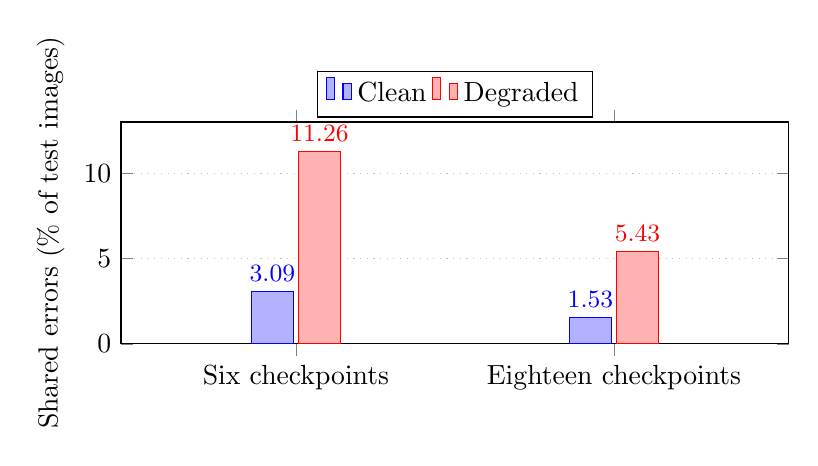
\begin{tikzpicture}
\begin{axis}[width=.83\linewidth,height=4.4cm,ybar,bar width=15pt,ymin=0,ymax=13,
 ylabel={Shared errors (\% of test images)},symbolic x coords={Six checkpoints,Eighteen checkpoints},
 xtick=data,legend style={at={(.5,1.02)},anchor=south,legend columns=2},
 nodes near coords,nodes near coords align={vertical},every node near coord/.append style={font=\small},
 enlarge x limits=.55,ymajorgrids=true,grid style={dotted}]
\addplot coordinates {(Six checkpoints,3.09) (Eighteen checkpoints,1.53)};
\addplot coordinates {(Six checkpoints,11.26) (Eighteen checkpoints,5.43)};
\legend{Clean,Degraded}
\end{axis}
\end{tikzpicture}
\caption{Descriptive shared-error fractions for two explicitly defined rosters. These are full-export counts, not estimates from the confusion-stratified 64-image explanation cohort. No causal interpretation or cross-dataset extrapolation is implied.}
\label{fig:shared}
\end{figure}

\subsection{Validation selection and the boundary of visual evidence}
The validation-only rule selects the DINO/RGB--log-magnitude pair. Its mean released RGB validation AUC is 0.993830 and its mean log-magnitude validation AUC is 0.851000; the mean RGB-to-frequency difference is 0.142830. The mean worst-domain criterion is 0.851000. These are selection statistics, not held-out evidence that frequency improves detection. They also do not imply that DINO has the best degraded-test RGB score, which Table~\ref{tab:auc} assigns to CLIP within this roster.

The reference-stratified 64-ID cohort and the primary 5,623-ID shared-error cohort can be frozen from the exports. However, authenticated MFFI image access was unavailable: the official download returned HTTP 401. Therefore \emph{no completed full-cohort heatmap comparison, attribution-quality ranking, spectral-cluster finding, or visual failure-cause result is reported here}. Technical implementation tests and checkpoint-loading checks are not substitutes for those experiments. Table~\ref{tab:boundary} makes the distinction explicit.

\begin{table}[t]
\centering
\caption{Evidence boundary at this revision. ``Defined'' is not ``experimentally completed.''}
\label{tab:boundary}
\small
\begin{tabular}{p{.56\linewidth}p{.34\linewidth}}
\toprule
Item & Status\\
\midrule
54 RGB prediction exports and validation curation & Reanalysed\\
Six- and eighteen-checkpoint shared-error counts & Computed\\
Reference-stratified 64-image IDs & Selected from exports\\
RGB--frequency pair selection & Computed from validation aggregates\\
Full-cohort source-image inference verification & Pending image access\\
Tasks 1--3 heatmaps and attribution controls & Pending image access and execution\\
Lighting, occlusion, or demographic failure causes & Not established\\
\bottomrule
\end{tabular}
\end{table}

\section{Limitations and completion requirements}
This audit uses one released dataset and checkpoint collection. Degraded MFFI evaluation is not cross-dataset generalization, and apparent family differences do not isolate architecture from pretraining or training choices. The legacy numeric-ID linkage and missing validation observation limit provenance until source images and original decode logs are checked. The disclosed derived validation view supports a reproducible recalibration, but it cannot restore the omitted image or certify that other preprocessing defects are absent.

The six-model explanation roster fixes seed 42 for tractability and comparability; it does not establish seed-invariant explanation behavior. The 18-model sensitivity analysis concerns prediction intersections, not completed multi-seed attribution. The 64-image cohort is deliberately outcome-stratified and unsuitable for population-level explanation claims. Label-matched hard-sample controls do not remove acquisition or demographic confounding. Parameter randomization, baseline sensitivity, and perturbation tests examine specific properties; passing them cannot certify that a model uses semantically correct or causal evidence.

To complete the image-dependent study, the authors must obtain authorized source-image access, verify the exact input bytes and exported probabilities, run all declared supported cells and controls, inspect coverage and failed cases, and report the resulting quality and computational statistics. Any causal or subgroup hypothesis requires additional annotations and an appropriate analysis plan. The earlier manuscript states acceptance at SIBGRAPI; its relationship to a proposed new submission requires author and venue-policy review. This document is not a claim of ICLR submission eligibility or a submission-ready completed XAI study.

\section{Conclusion}
An explanation pipeline cannot repair uncertain experimental provenance merely by producing more heatmaps. The released fine-tuned RGB predictions support a reproducible finding that clean and degraded rankings differ and that complete-roster shared failures increase substantially under degradation. They also expose a validation-export integrity defect that must be disclosed before calibrating decisions or selecting confusion strata. The proposed protocols fix the reference cohort, target, coordinate system, model roster, and evidence accounting, while withholding visual and causal claims that have not been measured. Completing the source-image experiments will determine whether any spatial or spectral attribution pattern survives these controls; it is not a conclusion of the present revision.

\section*{Ethics statement}
Face imagery can contain sensitive personal information. This revision does not infer identity, ethnicity, or skin-tone categories, and does not redistribute the gated MFFI image collection. Dataset availability or a repository license should not be treated as proof of consent for every downstream use. Detector errors and attribution maps must not be used as definitive evidence about a person's authenticity or conduct. The image-dependent follow-up requires authorized data access, appropriate annotation governance, and explicit uncertainty in forensic interpretation.

\section*{Reproducibility statement}
The accompanying code and research records identify the immutable source and model revisions, prediction files, manifest-order assumption, explicit validation curation, calibration rule, sampling seed, and complete model rosters. Appendix~\ref{app:reproduce} specifies the reconstruction boundary. Raw exports remain separate from derived artifacts. A completed run must record image and checkpoint hashes and reproduce the frozen predictions before attribution outputs enter the empirical analysis.

\section*{AI use statement}
An AI assistant was used for literature discovery, artifact inspection, programming, test development, numerical reanalysis, and drafting this revision. This assistance extends beyond spelling or stylistic editing. The research records distinguish executed calculations from proposed or blocked experiments. Human authors must independently review the code, sources, results, publication overlap, and manuscript, determine authorship and submission suitability, and accept responsibility for the final work. This revision has not yet received that author sign-off.

\bibliography{references}
\bibliographystyle{iclr2027_conference}

\appendix
\section{Reproducibility and completion checklist}\label{app:reproduce}
\paragraph{Pinned artifacts.}
The repository baseline is
\begin{quote}\small\texttt{1643db7a82f111f1a468dba986fe29593761b6be}.\end{quote}
The Hugging Face repository is \texttt{lucasoc/MFFI-Models}, pinned to
\begin{quote}\small\texttt{3bef179cdc08850e1d720182e55a040d00c9d582}.\end{quote}
Runs use the path convention \texttt{family/mode/regime/seed\_N/}, with configuration and prediction exports in \texttt{results/} and the full checkpoint in \texttt{weights/best.pth}. RGB is encoded by the release mode name \texttt{none}. Thresholds must be recomputed under the declared validation-curation policy rather than silently copied from differently calibrated summaries.

\paragraph{Identity contract.}
Retain the original manifest bytes and hash before assigning zero-based legacy IDs. Trim filename whitespace for path resolution without changing row order. Reject path traversal, duplicate source names, duplicate test IDs, inconsistent labels, non-finite probabilities, missing predictions, and incomplete rosters. Validation deduplication requires an explicit opt-in and identical repeated records. Store the missing-ID report and the derived validation manifest separately. Before attribution, verify source-image hashes and checkpoint/configuration hashes and compare fresh probabilities and decisions against the frozen cohort.

\paragraph{Attribution contract.}
Record model family, exact checkpoint, actual topology, training regime, representation, input size and channel count, preprocessing order, target layer or token reshape, fixed output target, method and library version, baseline and background, feature masks, random seed, numerical budget, raw signed output, convergence or degeneracy diagnostics, device and runtime, and artifact hashes. RGB zero in ImageNet-normalized coordinates denotes the normalization mean, not black. A frequency-domain zero baseline has a different meaning and must be labeled accordingly. Group-wise display densities are not individual-feature Shapley values.

\paragraph{Completion gate.}
A full Task 1 run contains all 64 frozen observations for every declared model and method, with explicit unsupported records. Task 2 uses the selected matched pair and the same source IDs; native domains must not be mislabeled or overlaid on unrelated coordinates. Task 3 contains every primary shared-error ID and its separately frozen controls. Failed image decoding must stop the run or be reported as a failure, never substitute another image. Resume and sharding must preserve the cohort and method contracts. Final visual conclusions require complete coverage, quality controls, sensitivity analyses, and human review; none can be inferred from this checklist alone.
\end{document}
